\documentclass{beamer}

\mode<presentation>

\usetheme{Copenhagen}
\usecolortheme{rose}
\setbeamercovered{transparent}

\usepackage[T1]{fontenc}
\usepackage[serbian]{babel}
\usepackage[utf8]{inputenc}

\usepackage{graphicx}
\usepackage{amsmath}

\title[GeoSerbia]
{GeoSerbia \\ Sistem za geografski kviz u Srbiji}

\author[A. Malezić]
{Aleksa Malezić \\ 24/3124}

\institute{
Projekat iz predmeta\\
Personalizovane Aplikacije\\
ETF
}

\date{2026}

\begin{document}

%------------------------------------------------

\begin{frame}
\titlepage
\end{frame}

%------------------------------------------------

\begin{frame}
\frametitle{Sadržaj}
\tableofcontents
\end{frame}

%------------------------------------------------
\section{Uvod}

\begin{frame}
\frametitle{Ideja sistema}

GeoSerbia je web aplikacija inspirisana GeoGuessr igrom.

\begin{block}{Cilj aplikacije}
Igrač dobija fotografiju lokacije u Srbiji i treba da pogodi
njenu poziciju na mapi.
\end{block}

\begin{itemize}
\item igra zasnovana na geografskom znanju
\item fotografije realnih lokacija
\item bodovanje prema udaljenosti
\item dnevni i mesečni leaderboard
\end{itemize}

\end{frame}

%------------------------------------------------
\section{Arhitektura sistema}

\begin{frame}
\frametitle{Arhitektura sistema}

\begin{figure}
\centering
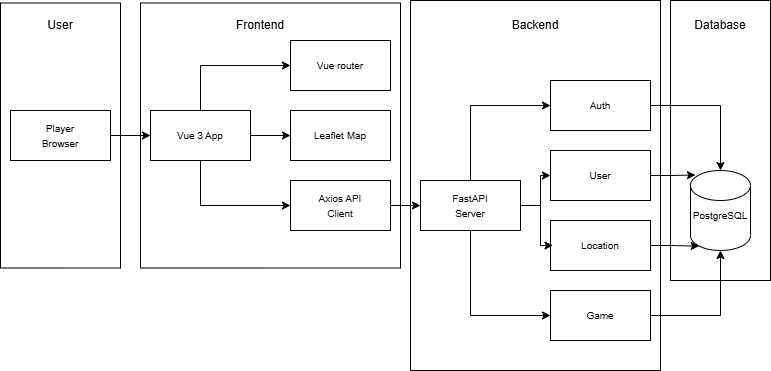
\includegraphics[width=0.85\textwidth]{architecture_diagram.png}
\end{figure}

\begin{itemize}
\item klijent–server arhitektura
\item frontend aplikacija komunicira sa backend API-jem
\item backend pristupa PostgreSQL bazi
\end{itemize}

\end{frame}

%------------------------------------------------
\section{Tehnologije}

\begin{frame}
\frametitle{Backend tehnologije}

\begin{itemize}
\item FastAPI
\item PostgreSQL
\item Tortoise ORM
\item Aerich migracije
\item JWT autentifikacija
\item Pytest test framework
\end{itemize}

\end{frame}

%------------------------------------------------

\begin{frame}
\frametitle{Frontend tehnologije}

\begin{itemize}
\item Vue 3 (Composition API)
\item Vue Router
\item Axios
\item Leaflet mapa
\item Vite build alat
\end{itemize}

\end{frame}

%------------------------------------------------
\section{Baza podataka}

\begin{frame}
\frametitle{Model baze podataka}

\begin{figure}
\centering
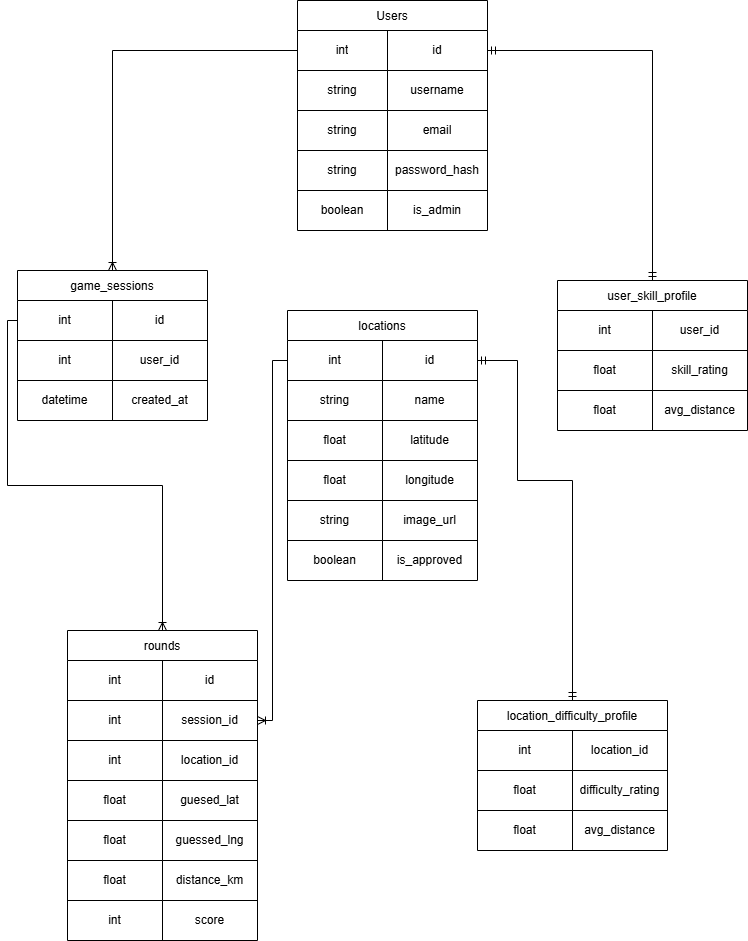
\includegraphics[width=0.85\textwidth]{database_er_diagram.png}
\end{figure}

\end{frame}

%------------------------------------------------
\section{Gameplay}

\begin{frame}
\frametitle{Tok igre}

\begin{itemize}

\item korisnik pokreće igru
\item sistem bira lokaciju
\item igrač bira tačku na mapi
\item backend računa udaljenost
\item rezultat se prikazuje korisniku

\end{itemize}

\end{frame}

%------------------------------------------------

\begin{frame}
\frametitle{Računanje udaljenosti}

Udaljenost između dve geografske tačke računa se
Haversine formulom:

\[
d = 2R \arcsin
\left(
\sqrt{
\sin^2\left(\frac{\phi_2-\phi_1}{2}\right)
+
\cos(\phi_1)\cos(\phi_2)
\sin^2\left(\frac{\lambda_2-\lambda_1}{2}\right)
}
\right)
\]

\begin{itemize}
\item $\phi$ – geografska širina
\item $\lambda$ – geografska dužina
\item $R$ – poluprečnik Zemlje
\end{itemize}

\end{frame}

%------------------------------------------------
\section{Request flow}

\begin{frame}
\frametitle{Tok zahteva kroz sistem}

\begin{figure}
\centering
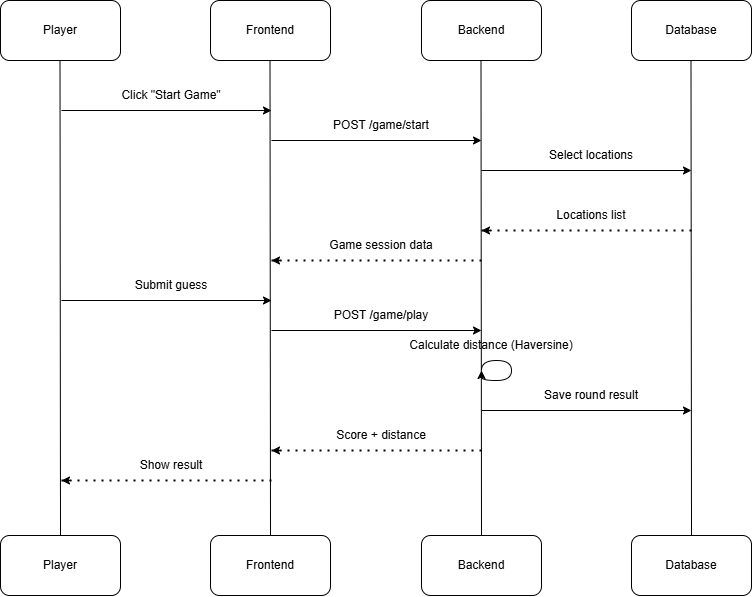
\includegraphics[width=0.9\textwidth]{flow_diagram.png}
\end{figure}

\end{frame}

%------------------------------------------------
\section{Adaptivni sistem}

\begin{frame}
\frametitle{Adaptivni sistem težine}

Sistem prati performanse korisnika i prilagođava težinu igre.

\begin{block}{Modeli}
\begin{itemize}
\item user\_skill\_profile
\item location\_difficulty\_profile
\item adaptive\_decision\_log
\end{itemize}
\end{block}

Adaptive mod bira lokacije koje najbolje odgovaraju
trenutnom nivou znanja korisnika.

\end{frame}

%------------------------------------------------
\section{Zaključak}

\begin{frame}
\frametitle{Zaključak}

GeoSerbia predstavlja full-stack sistem za implementaciju
geografske igre.

\begin{itemize}

\item backend implementiran u FastAPI
\item frontend u Vue 3
\item PostgreSQL baza podataka
\item adaptivni sistem težine
\item leaderboard i statistika korisnika

\end{itemize}

\end{frame}

%------------------------------------------------

\begin{frame}
\centering
\Huge Hvala na pažnji
\end{frame}

\end{document}